%%
%% This is file `mcmthesis-demo.tex',
%% generated with the docstrip utility.
%%
%% The original source files were:
%%
%% mcmthesis.dtx  (with options: `demo')
%% 
%% -----------------------------------
%% 
%% This is a generated file.
%% 
%% Copyright (C)
%%     2010 -- 2015 by Zhaoli Wang
%%     2014 -- 2016 by Liam Huang
%% 
%% This work may be distributed and/or modified under the
%% conditions of the LaTeX Project Public License, either version 1.3
%% of this license or (at your option) any later version.
%% The latest version of this license is in
%%   http://www.latex-project.org/lppl.txt
%% and version 1.3 or later is part of all distributions of LaTeX
%% version 2005/12/01 or later.
%% 
%% This work has the LPPL maintenance status `maintained'.
%% 
%% The Current Maintainer of this work is Liam Huang.
%% 
\documentclass{mcmthesis}

\mcmsetup{CTeX = false,   % 使用 CTeX 套装时,设置为 true
        tcn = {Yucheng Jin, Anbang Ye}, problem = A,
        sheet = true, titleinsheet = true, keywordsinsheet = true,
        titlepage = false, abstract = false}
\usepackage{gensymb}
\usepackage{graphicx,float}
\usepackage{palatino}
\usepackage[stable]{footmisc}
\usepackage{lipsum}
\usepackage{booktabs,siunitx}
\usepackage{amsthm}
\usepackage{lastpage}
\usepackage{fancyhdr}
\usepackage{array}
\usepackage{setspace}
\usepackage{textcomp}
\cfoot{\thepage}
\title{When "Spring" Comes to North Atlantic}

\begin{document}



\begin{center}


\item
\item

\huge{ECE 448} 

\huge{FA 2020}



\Large{Prof. Hongwei Wang}

\end{center}

\begin{center}

\item
\item
\item
\Huge{Assignment 1 Report}



\Huge{Search Algorithms}

\end{center}

\begin{center}

\item
\item
\item
\Large{Name: Yucheng Jin}
\item
\Large{ID: \qquad 3170112253}
\item
\Large{Name: \text{ } Yiqing Xie}
\item
\Large{ID: \qquad 3170111404}
\item
\Large{Name: Hangtao Jin}
\item
\Large{ID: \qquad 3170112247}
\item
\Large{Date: \text{ } Sept. 30, 2020}


\end{center}

\pagebreak
\renewcommand{\contentsname}{\tiny{}}
\begin{center}
\textbf{\Large{Table of Contents}}
\end{center}
\tableofcontents
\pagebreak
\section{Section I}

\subsection{BFS}
BFS means the breadth-first search algorithm. It uses a queue structure to realize its function. Queue is a first-in-first-out data structure, its \textit{enqueue} function inserts a new item at the top of the queue, and its \textit{dequeue} function removes the item at the top of the queue. BFS is a uniform cost search algorithm that guarantees optimal in the given scenario, because it expends uniformly until it detects the object. Beginning with the start point, BFS will search the neighbors of each point. When a new point is reached, BFS will mark it as "visited", and the next time when the point is reached again, BFS simply continues. We use a list to resemble the behavior of the queue, and another list to trace the points visited to realize BFS.\\
\\
1. State: means the characteristics of a point (e.g. whether it is an objective point).
\\
\\
2. Node: means the coordinates of a point (e.g. (x, y)).
\\
\\
3. Frontier: the set of neighbor points of the current point.
\\
\\
4. We trace the explored states by a list in python.
\\
\\
5. We ignore the repeated states.
\subsection{DFS}
DFS means the depth-first search algorithm. It uses a stack structure to realize its function. Stack is a first-in-last-out data structure, its \textit{push} function inserts a new item at the top of the stack, and its \textit{pull} function removes the item at the bottom of the stack. Beginning with the start point, BFS will search the neighbors of each point, and let the first neighbor point detected but not visited as the new start point. The same procedure will be repeated until the objective point is found. \\
\\
1. State: means the characteristics of a point (e.g. whether it is an objective point).
\\
\\
2. Node: means the coordinates of a point (e.g. (x, y)).
\\
\\
3. Frontier: the set of neighbor points of the current point.
\\
\\
4. We trace the explored states by a list in python.
\\
\\
5. We ignore the repeated states.
\subsection{Greedy}
Greedy best first search means that for each step, we want to get as closer as possible to the goal. When moving, we have four neighbors: up, down, left, right. We choose the position that is nearest to the goal.\\ 
\\
During each step, our current state includes the current coordinates and current Manhattan distance to the goal. Our node is the same as a state. Our frontier is all neighbors of the current point. When we want to take an item from the frontier, we will take the one with the least Manhattan distance to the goal. Each time we add a new point into our queue, we will calculate its Manhattan distance to the goal and insert it into the queue according this value. We don’t maintain an explored states list. However, we do store where the visited node comes from, which means the node who puts the visited node into the queue as a neighbor. When we go to the visited node next time, we will find it already has a “father”, then we can simply skip it.
\subsection{A*}
A* search arranges nodes waiting to be examined by f(n) = g(n) + h(n), which means the Manhattan distance to the goal plus the path length it already has gone through. Our current state includes current position, passed path length, and Manhattan distance to the goal. Our node is the same as state. Our frontier is all possible next points to be explored. We will take the one with least f(n) to be our next node. Just like the above Greedy solution, we do not maintain an explored state list, but only a list of “father” modes. When we meet a new point with father, we will see whether the new path has a smaller f(n). if so, we will update the point.
\pagebreak
\section{Section II}
For greedy BFS search, the heuristics is just the Manhattan distance to the goal. When we select the next state from frontier, we will choose the one with least heuristics. \\
\\
For A* search, the heuristics for single dot and multiple-dot situations are kind of different (though they use the same code). The code of A* search has two parts. The first part finds the path between the two assigned points. The single dot situation is solved by sorely using this part. In this part, the heuristics is the passed path length plus the Manhattan distance to the goal. To show that this is admissible, we can see that for all points, the remaining path length must be longer or equal to the Manhattan distance to the goal. As the real path that is equal to the passed path length plus the remaining pass length, it must be longer or be equal to the passed path length plus the Manhattan distance to the goal. So the heuristics is admissible for single dot situation. \\
\\
For the multiple-dot situation, the calculation is a lot more complex. We first calculate all path between any two points in the objectives. That means we will get a complete graph. Our second part of A* search is to find the shortest path that connects all vertices in the graph. We start from the start point and keep going to the next vertex until all vertices are connected. To choose the next vertex, we have our heuristics equal to the passed path length plus the edge between the current vertex and the next vertex plus the length of the MST (minimum spanning tree) of all remaining vertices (including the next vertex). We prove this heuristic is admissible below: the passed path length plus the edge between the current vertex and the next vertex is the path length between the start point and the next vertex. The length of the MST is always smaller than the remaining path length between the next vertex and the end vertex (though we don’t know which vertex is the end vertex yet). That means the sum of the values mentioned above, which is our heuristics, is always smaller than the real path, which equals to the path length between the start point and the next vertex plus the remaining path.

\pagebreak
\section{Section III}
\subsection{BFS}

\subsubsection{mediumMaze.txt}
Path Length: 111 \\ \\
States Explored: 661
\begin{center}
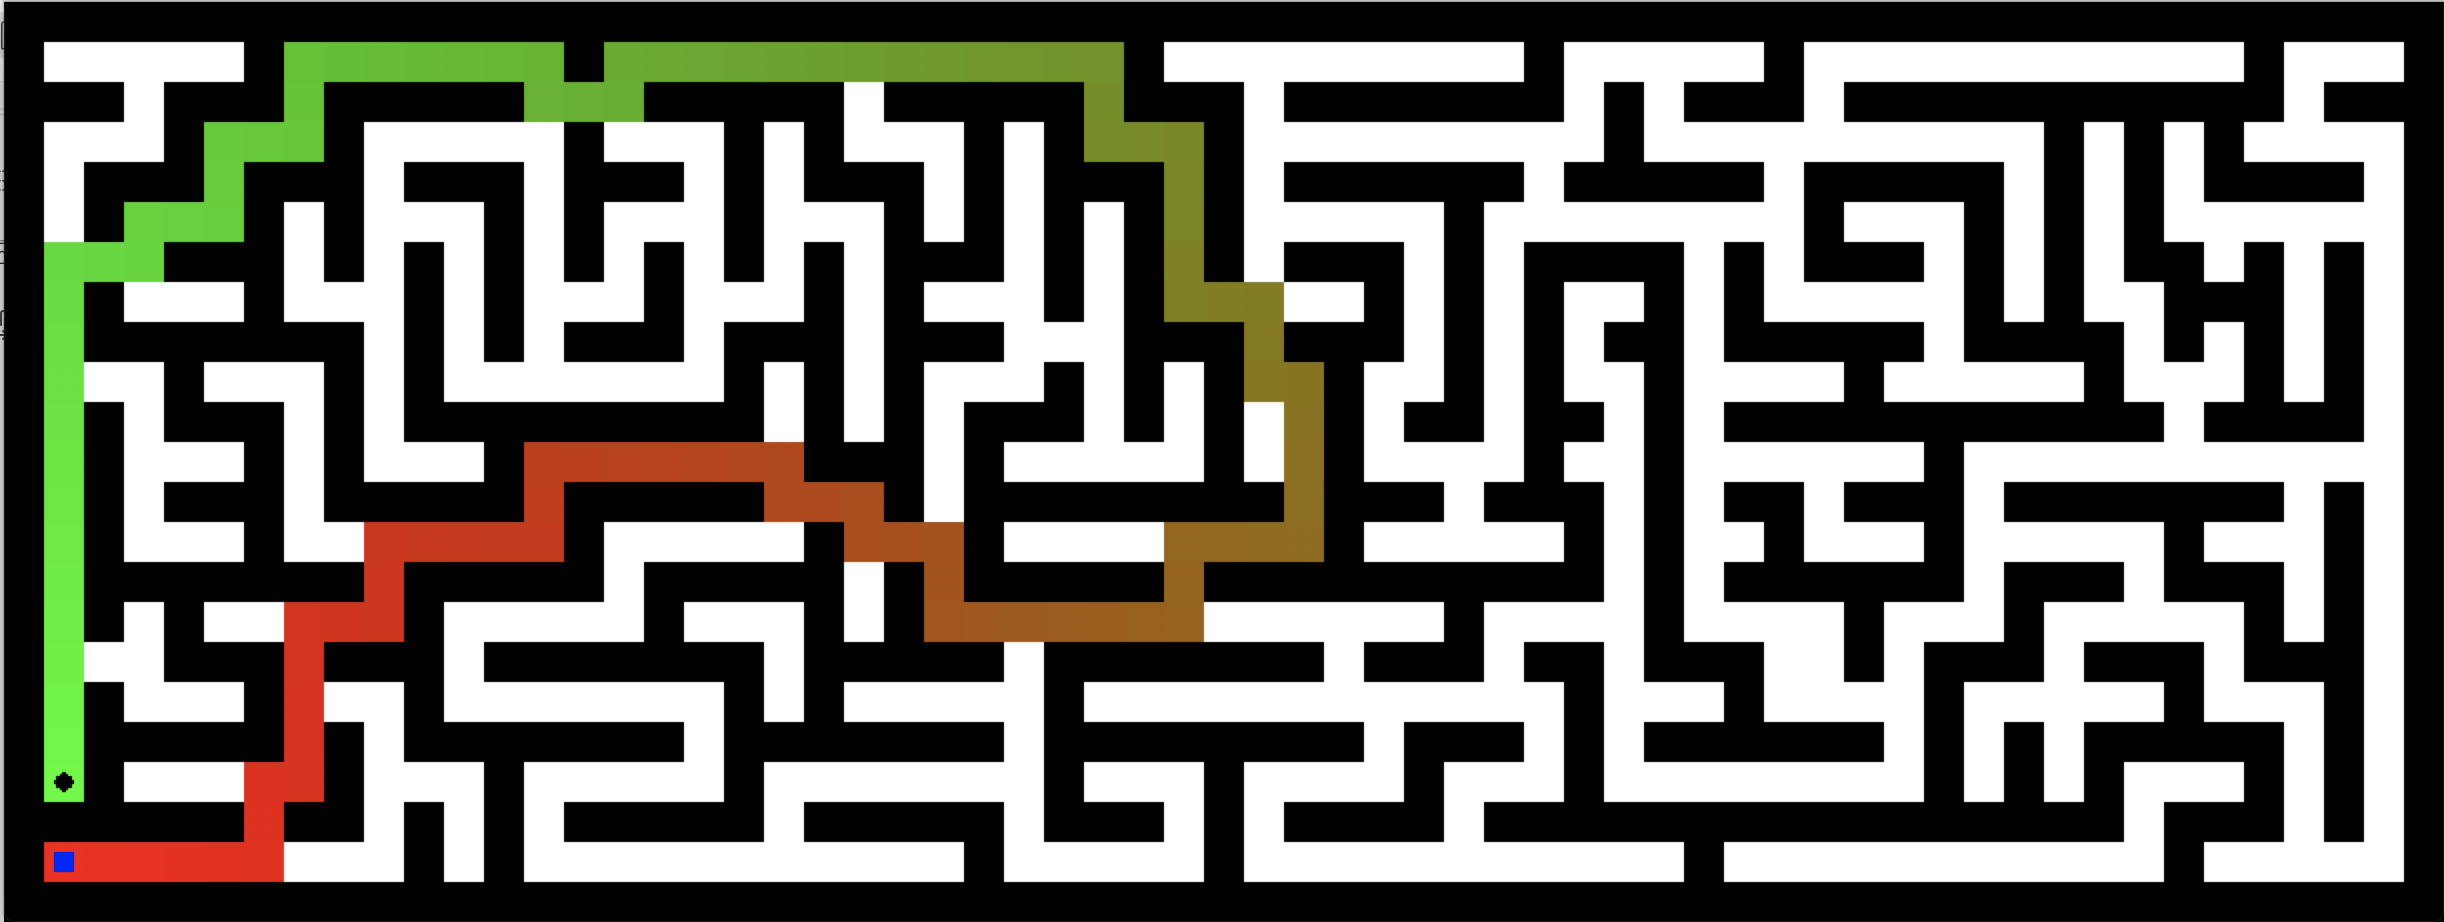
\includegraphics[width=15cm]{bfs_mediummaze.png}
\end{center}
\begin{center}
\small{Figure 3.1.1. BFS Solution for mediumMaze.txt}
\end{center}

\subsubsection{bigMaze.txt}
Path Length: 183 \\ \\
States Explored: 1422
\begin{center}
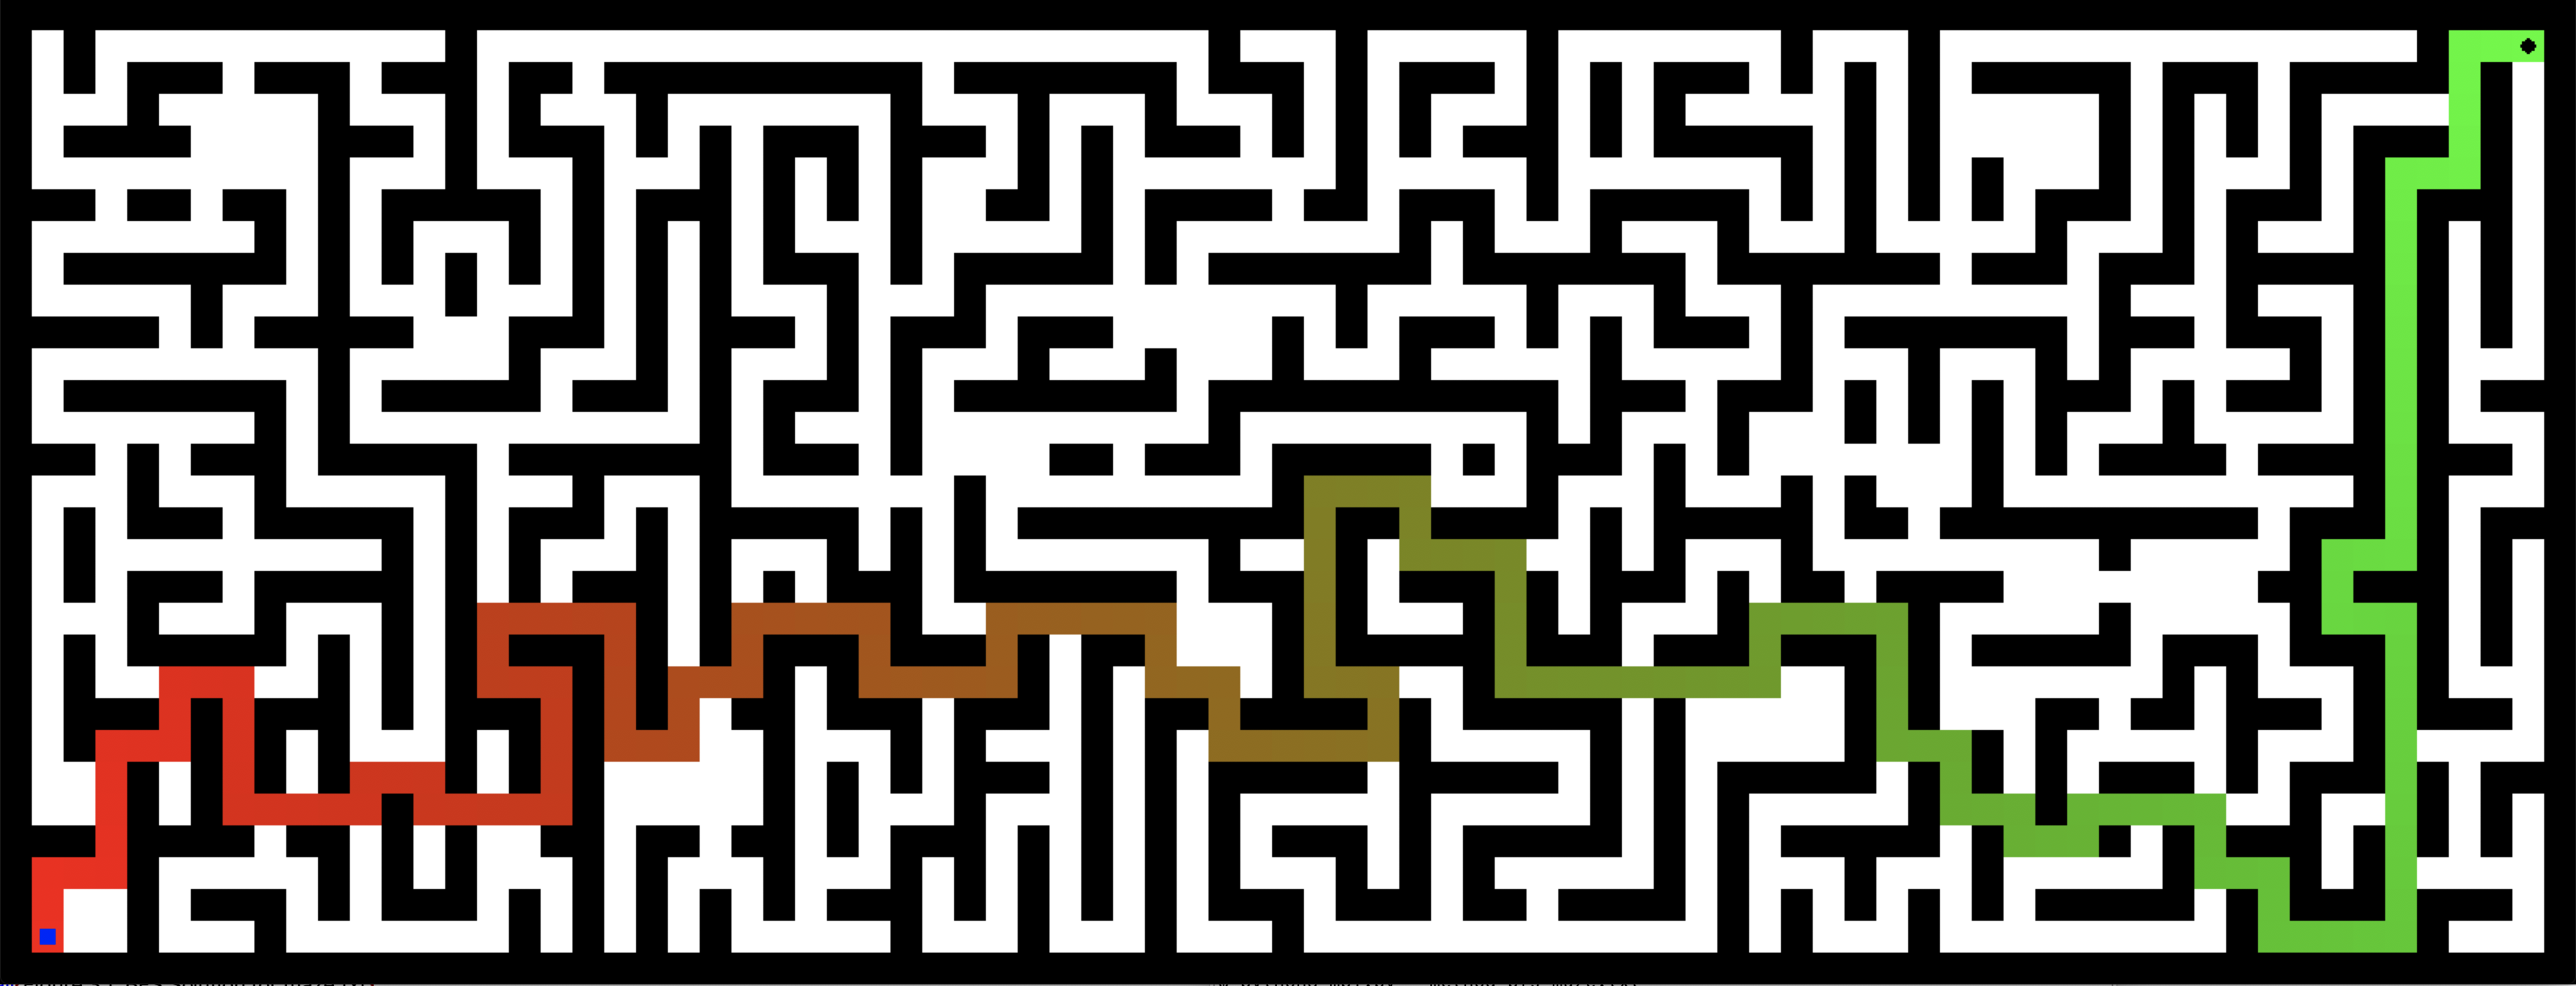
\includegraphics[width=15cm]{bfs_bigmaze.png}
\end{center}
\begin{center}
\small{Figure 3.1.2. BFS Solution for bigMaze.txt}
\end{center}

\subsubsection{openMaze.txt}
Path Length: 52 \\ \\
States Explored: 1019
\begin{center}

\includegraphics[width=12.5cm]{bfs_openmaze.png}
\end{center}
\begin{center}
\small{Figure 3.1.3. BFS Solution for openMaze.txt}
\end{center}

\subsection{DFS}

\subsubsection{mediumMaze.txt}
Path Length: 115 \\ \\
States Explored: 647
\begin{center}
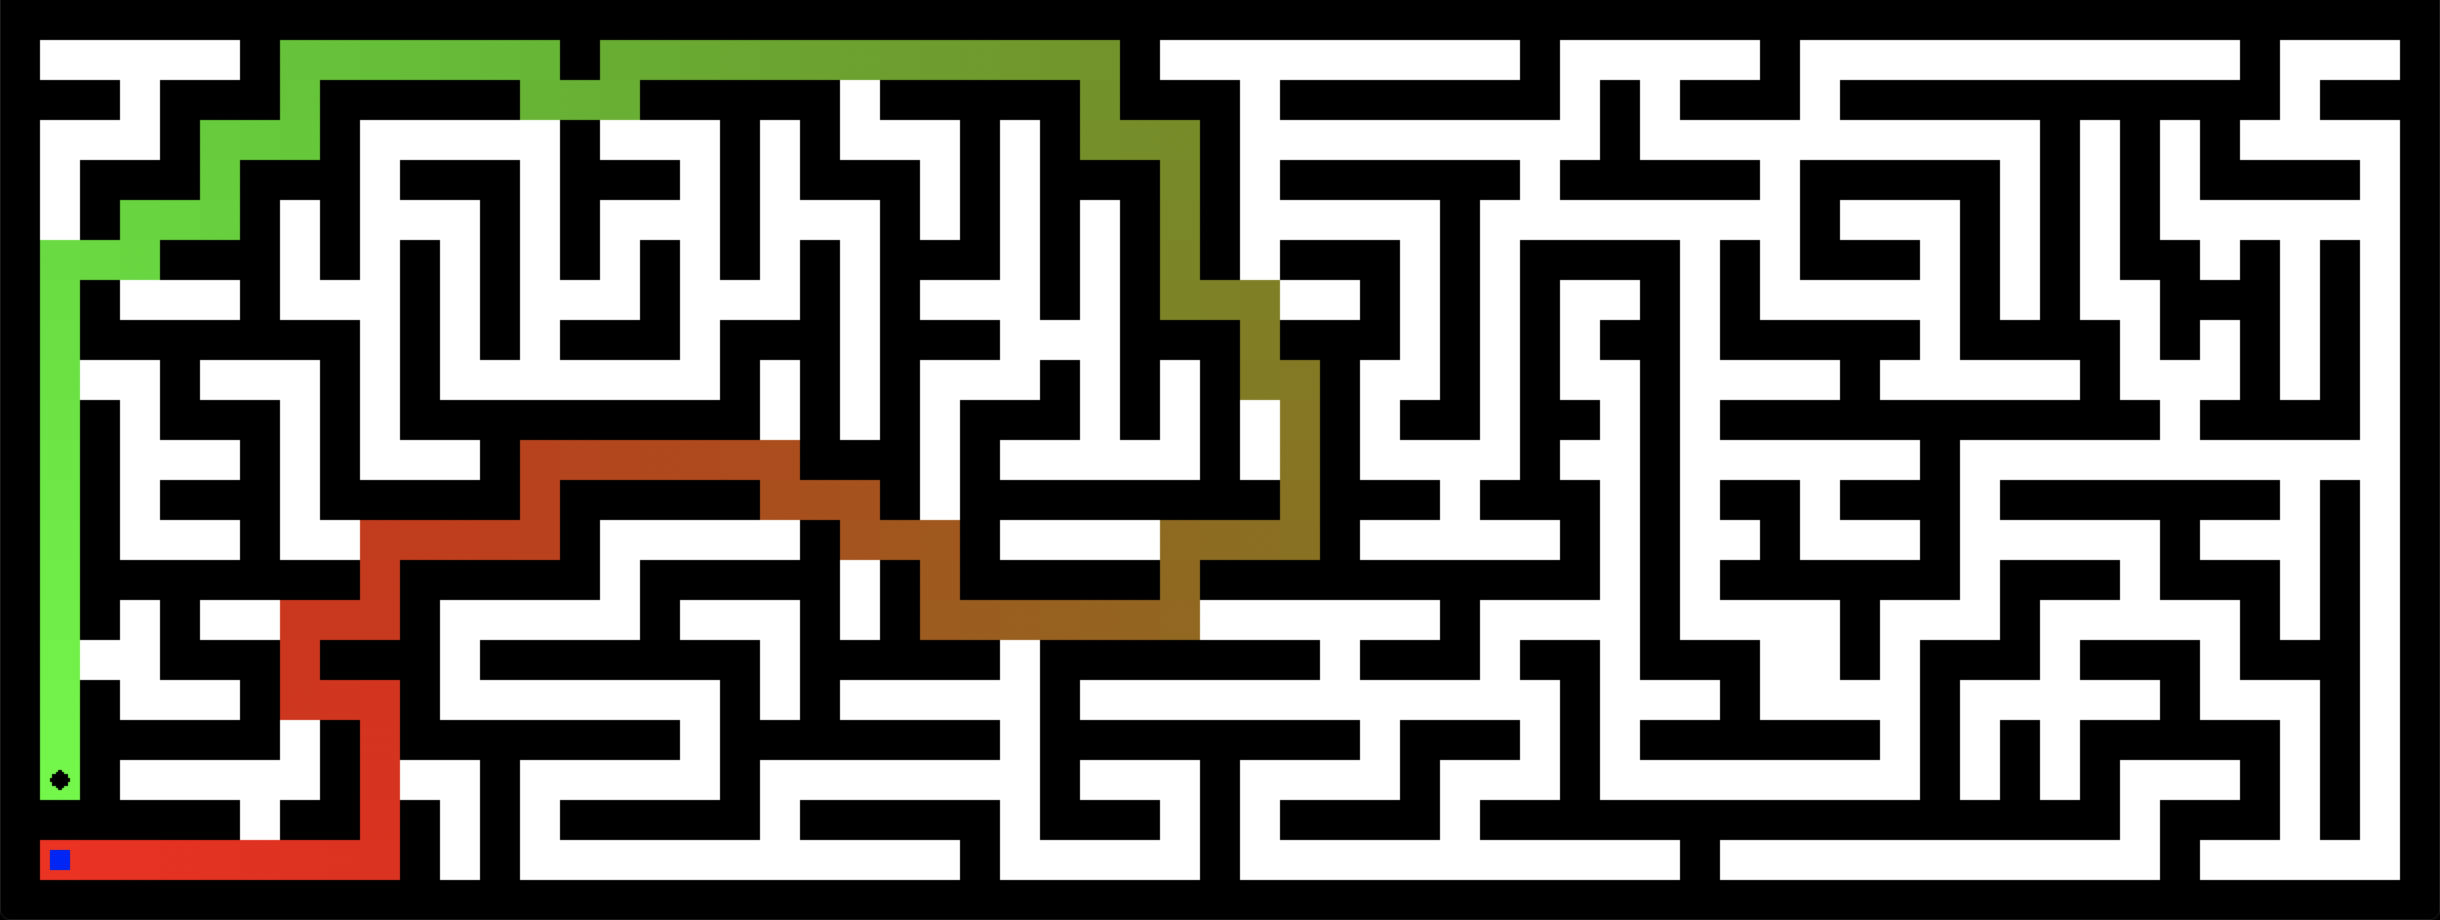
\includegraphics[width=15cm]{dfs_mediummaze.png}
\end{center}
\begin{center}
\small{Figure 3.2.1. DFS Solution for mediumMaze.txt}
\end{center}

\subsubsection{bigMaze.txt}
Path Length: 183 \\ \\
States Explored: 1287
\begin{center}
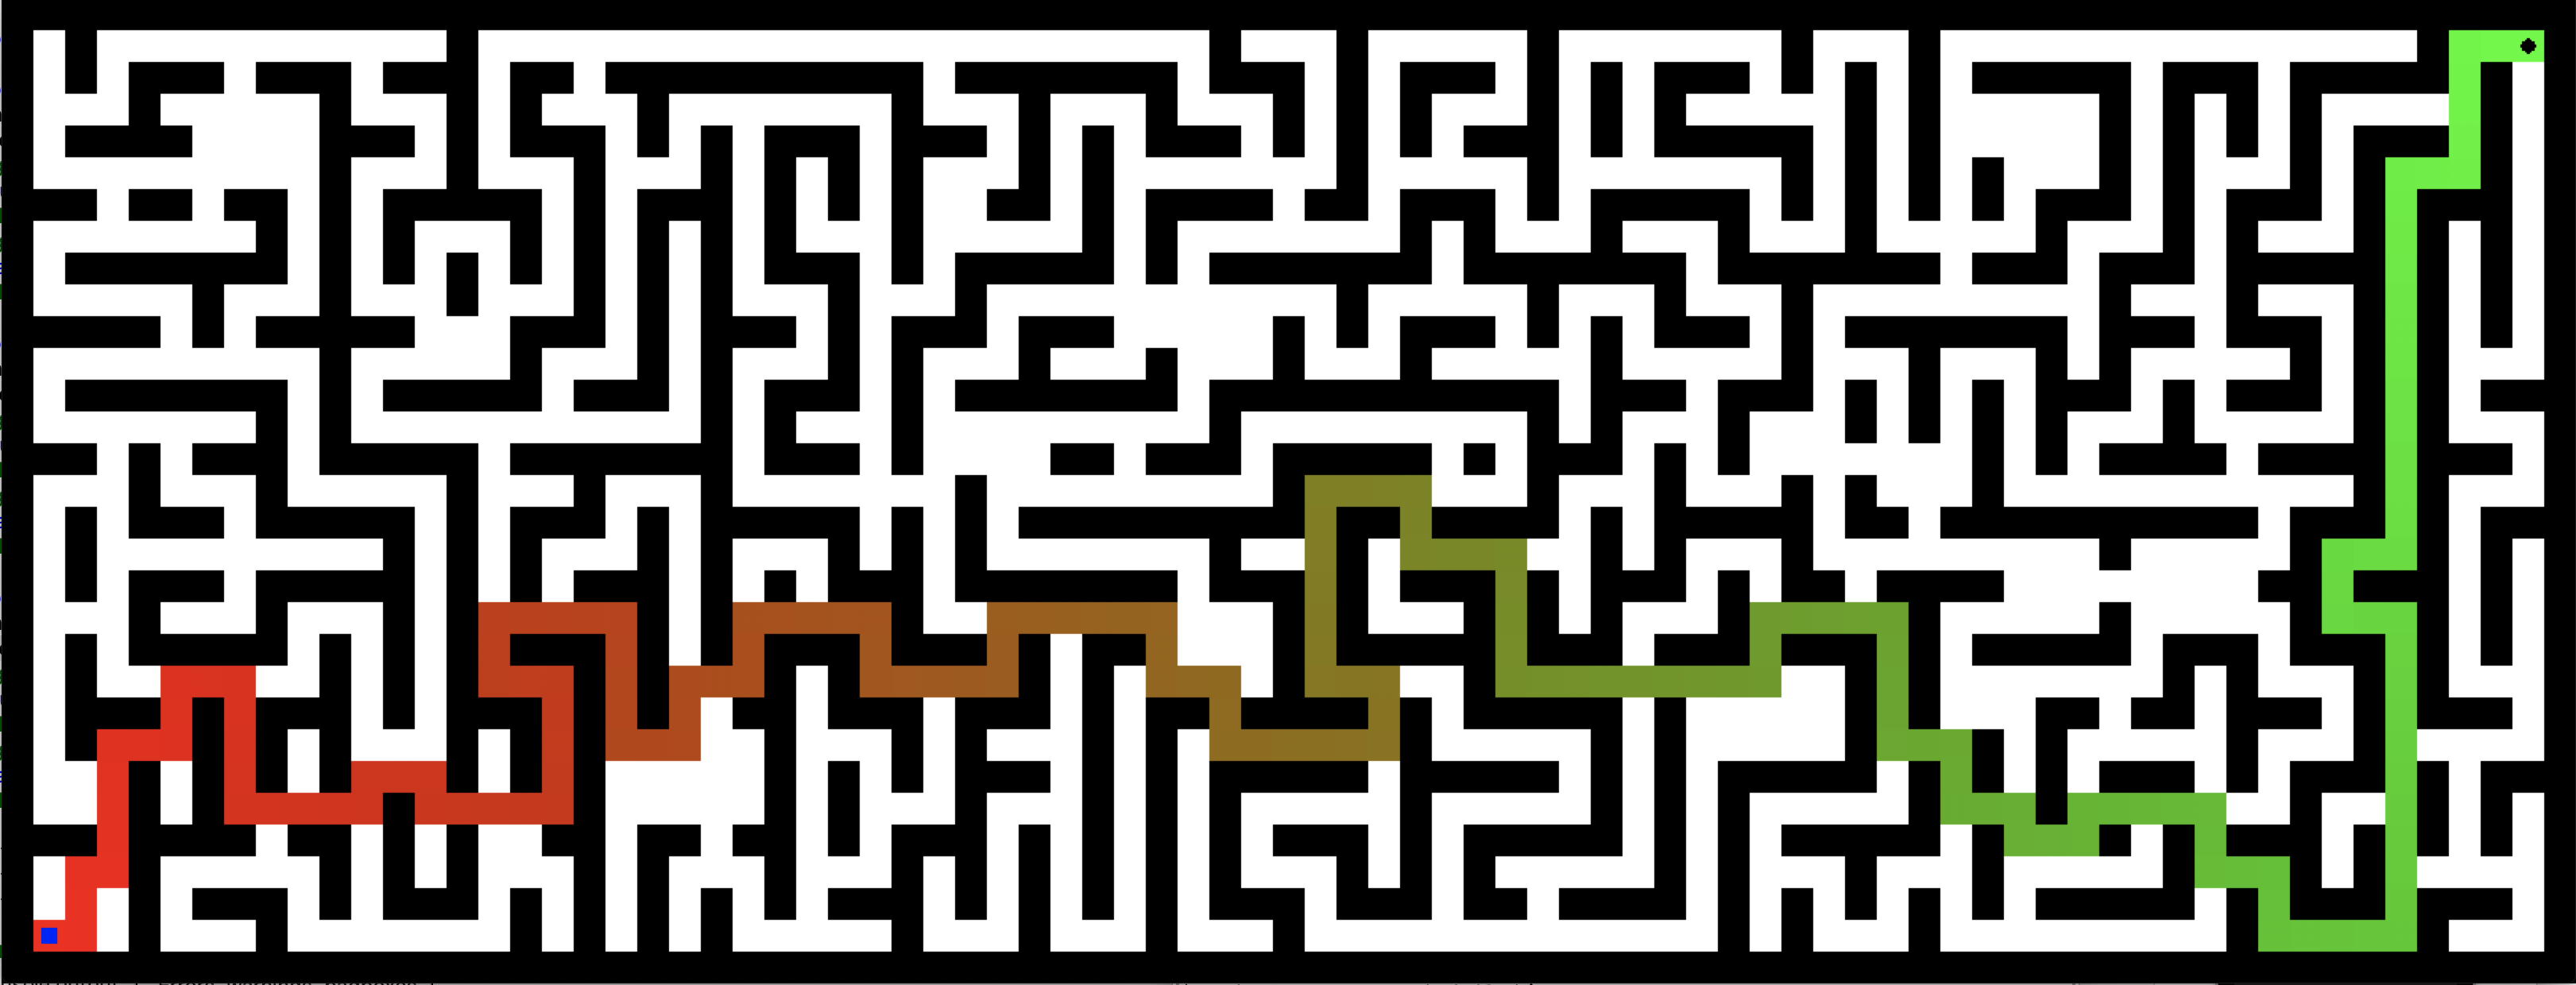
\includegraphics[width=15cm]{dfs_bigmaze.png}
\end{center}
\begin{center}
\small{Figure 3.2.2. DFS Solution for bigMaze.txt}
\end{center}

\subsubsection{openMaze.txt}
Path Length: 52 \\ \\
States Explored: 562
\begin{center}
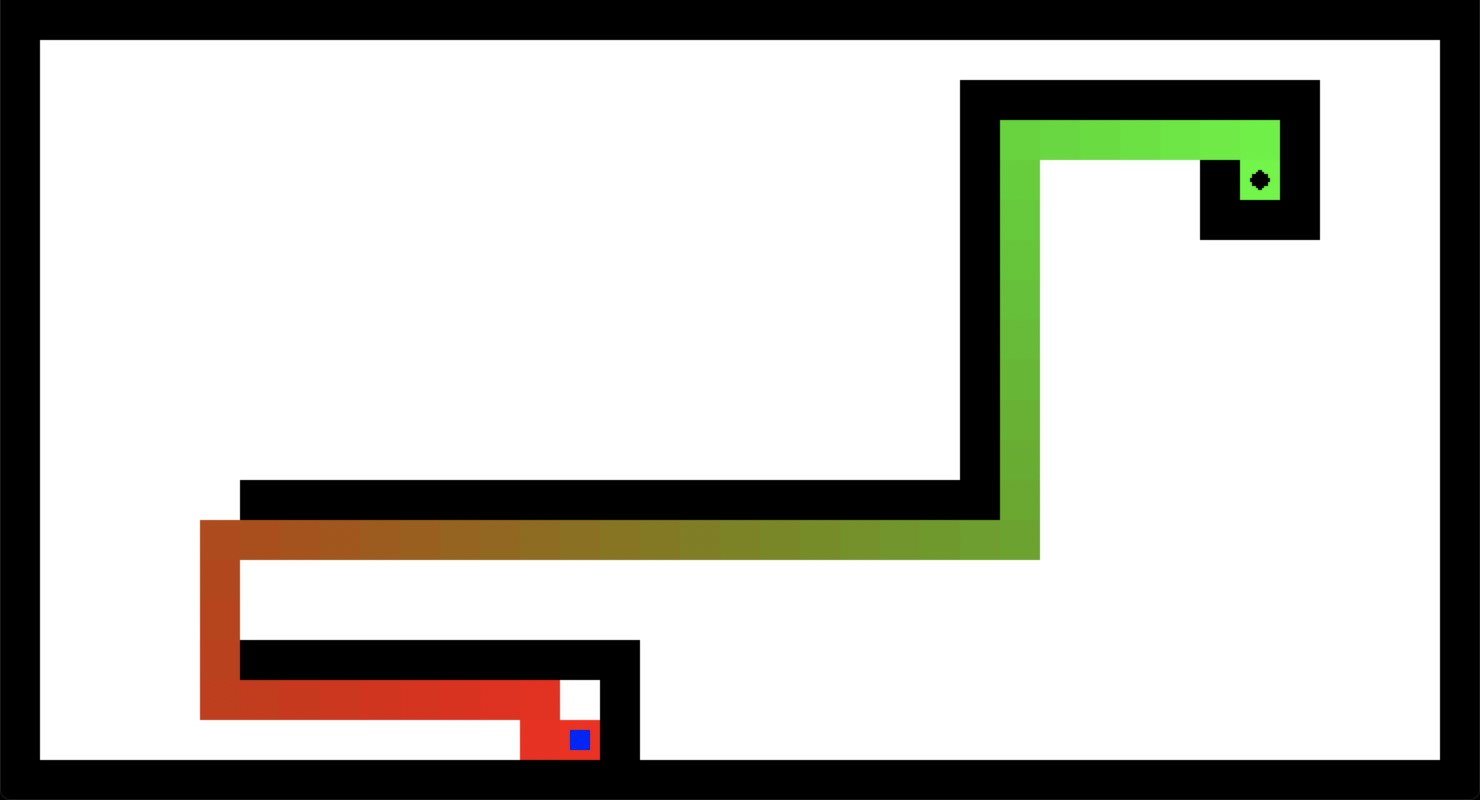
\includegraphics[width=12.5cm]{dfs_openmaze.png}
\end{center}
\begin{center}
\small{Figure 3.2.3. DFS Solution for openMaze.txt}
\end{center}

\subsection{Greedy}

\subsubsection{mediumMaze.txt}
Path Length: 147 \\ \\
States Explored: 343
\begin{center}
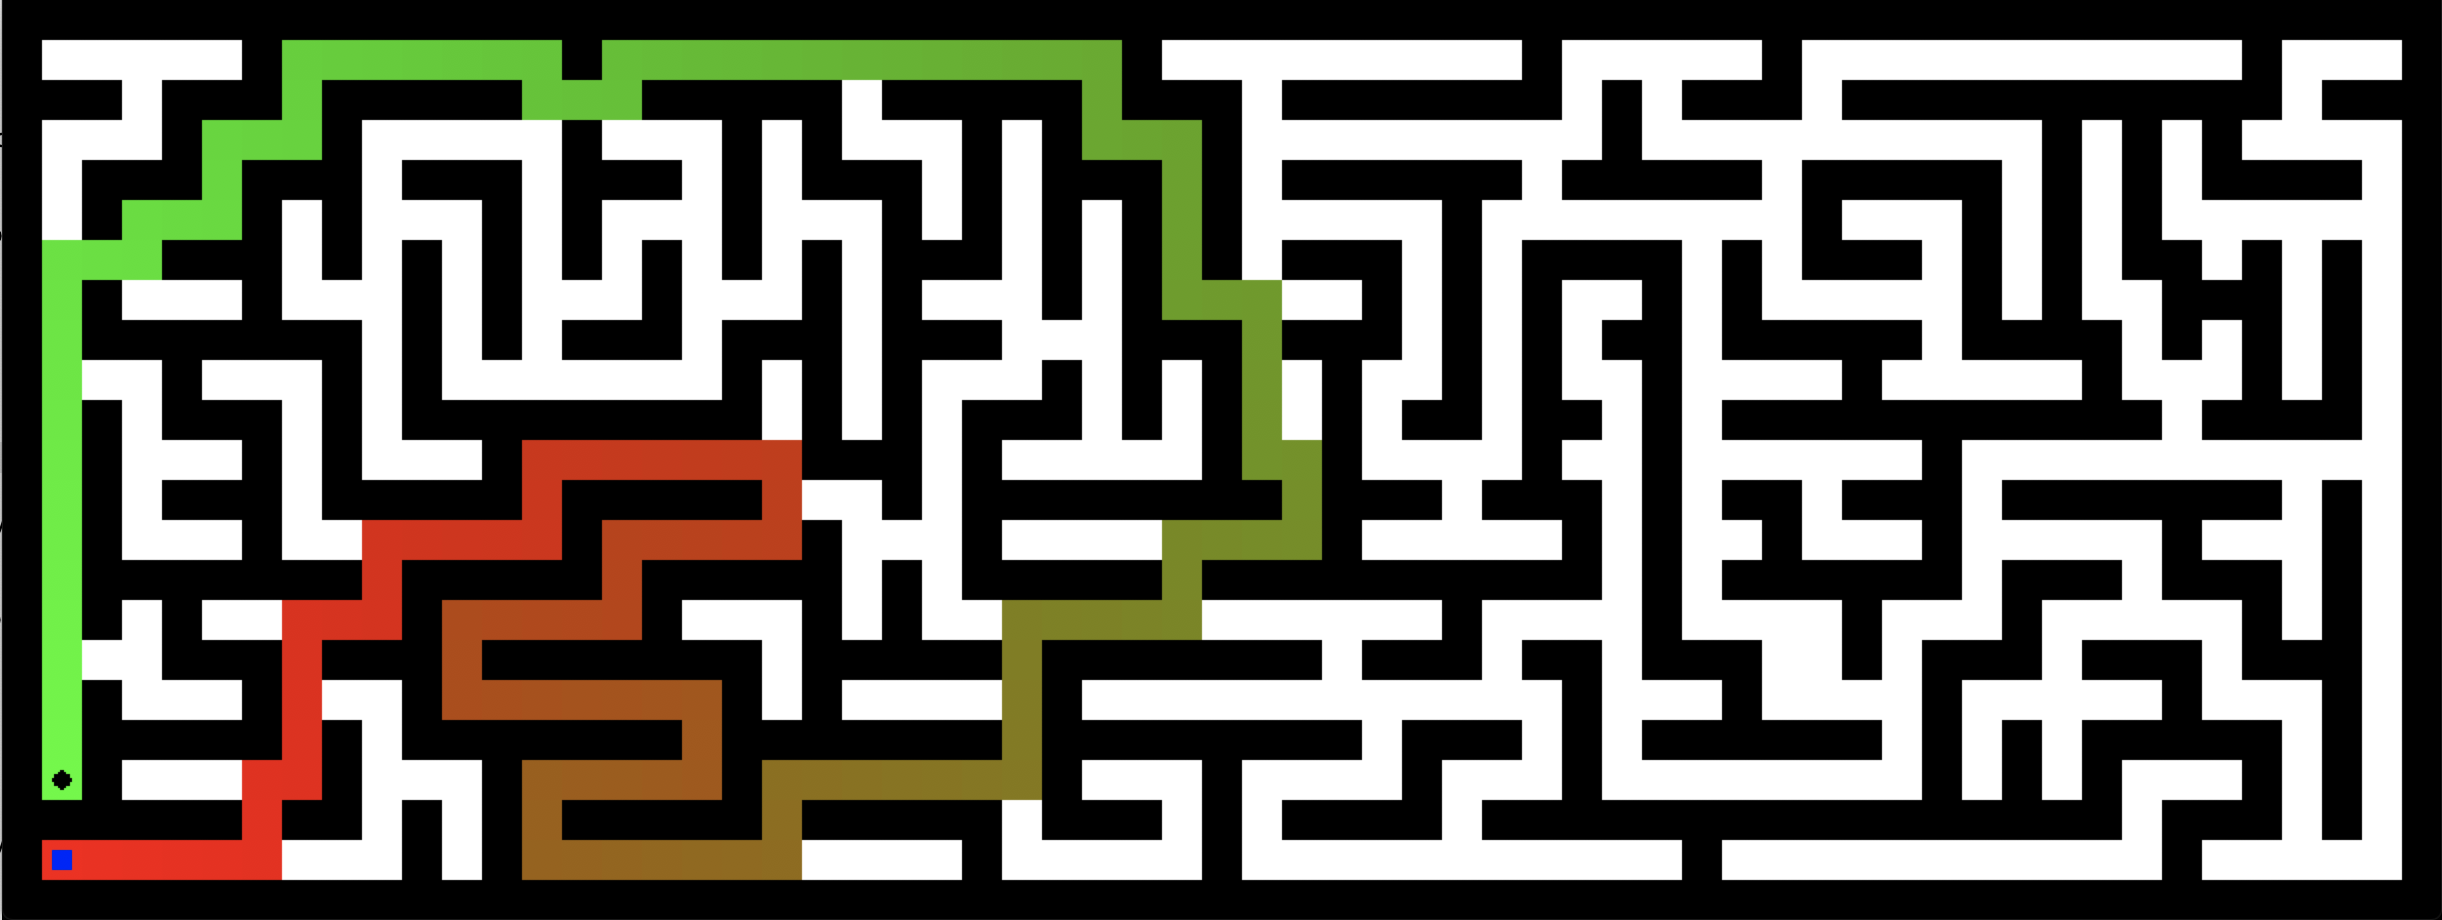
\includegraphics[width=15cm]{greedy_mediummaze.png}
\end{center}
\begin{center}
\small{Figure 3.3.1. Greedy Solution for mediumMaze.txt}
\end{center}

\subsubsection{bigMaze.txt}
Path Length: 277 \\ \\
States Explored: 468
\begin{center}
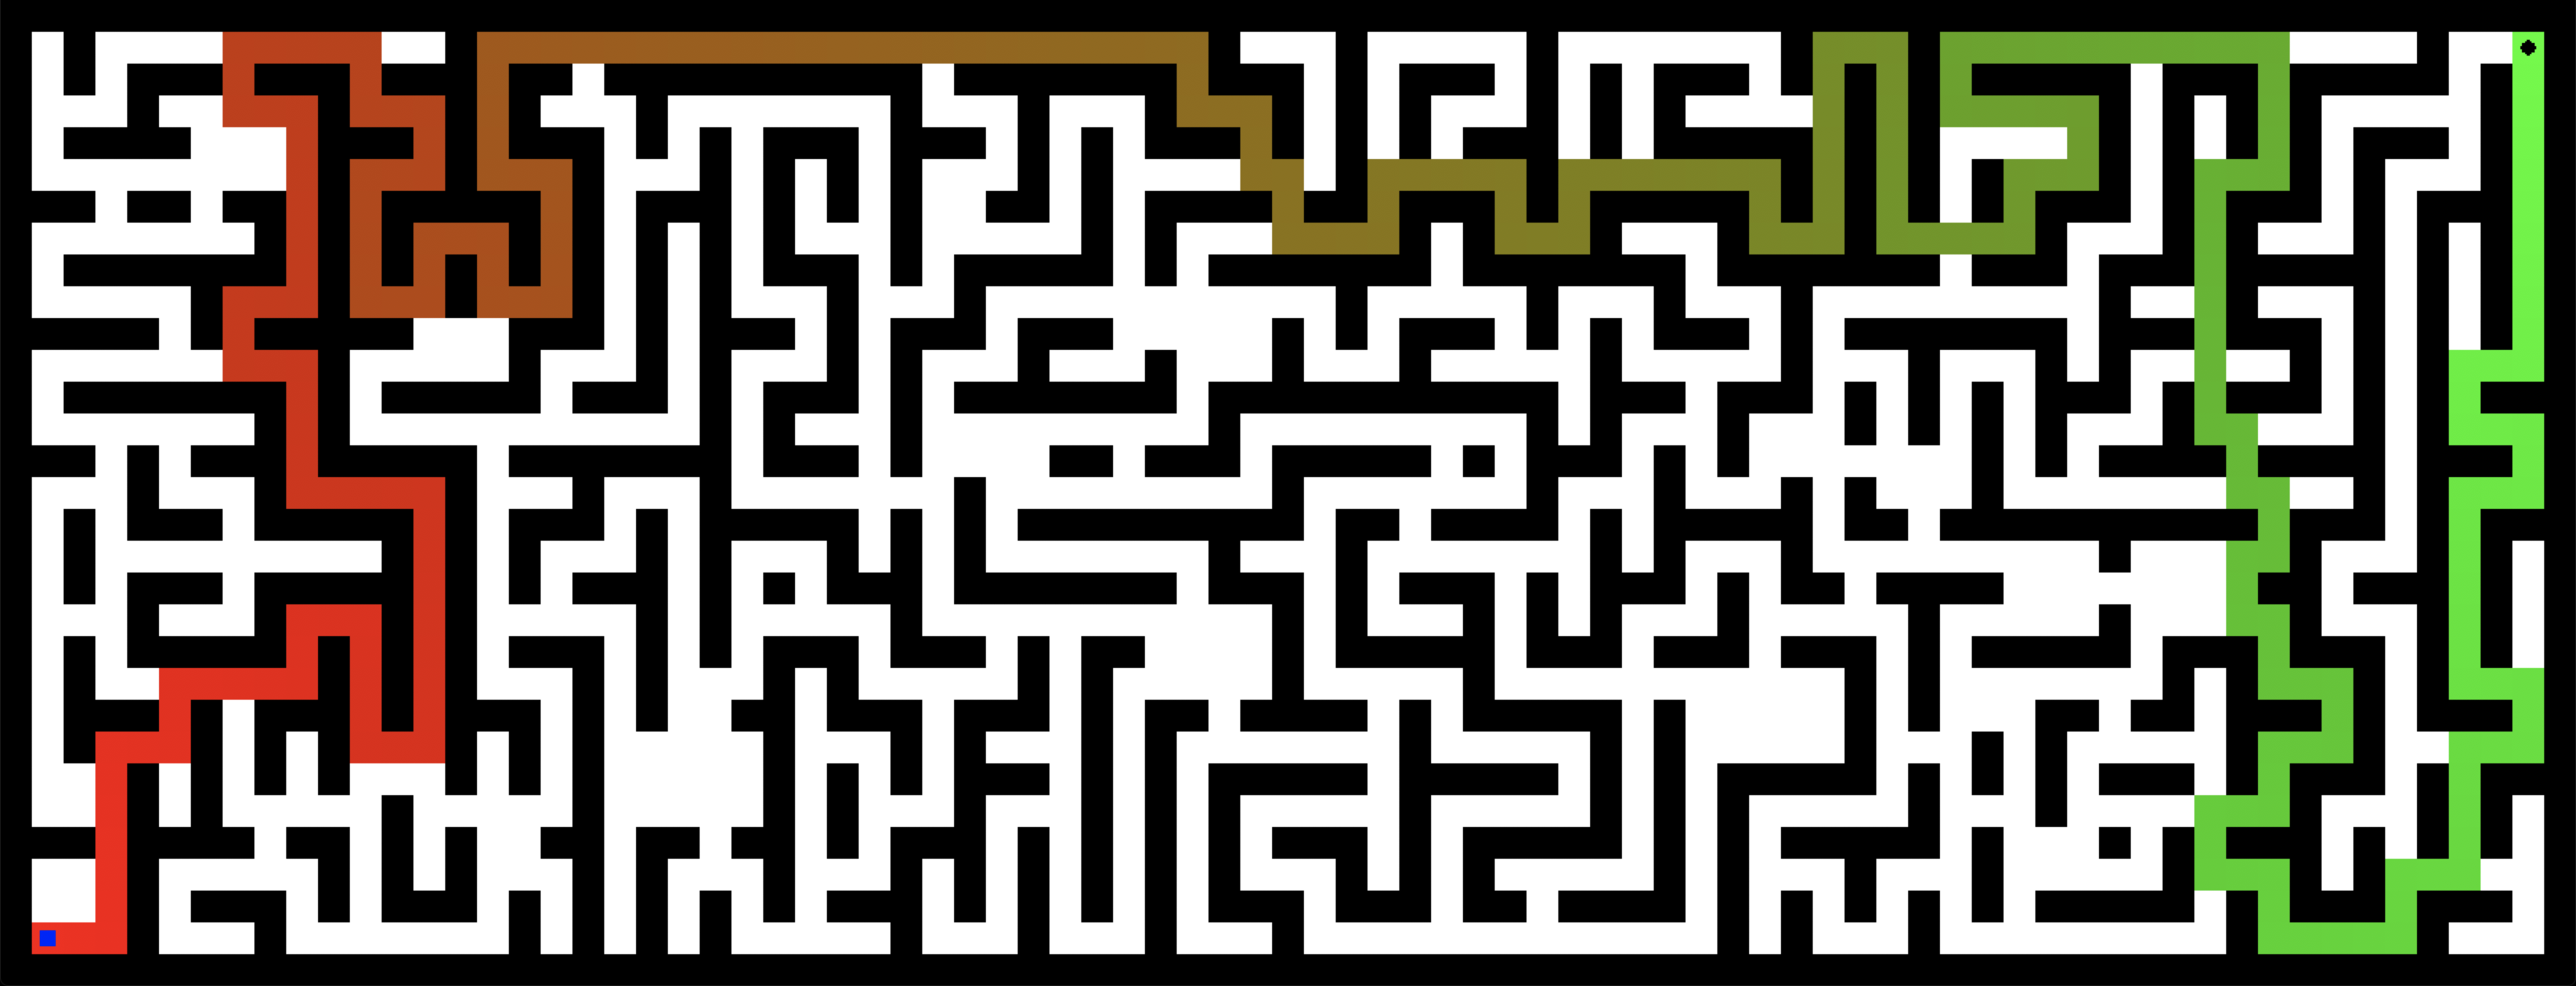
\includegraphics[width=15cm]{greedy_bigmaze.png}
\end{center}
\begin{center}
\small{Figure 3.3.2. Greedy Solution for bigMaze.txt}
\end{center}

\subsubsection{openMaze.txt}
Path Length: 56 \\ \\
States Explored: 74
\begin{center}
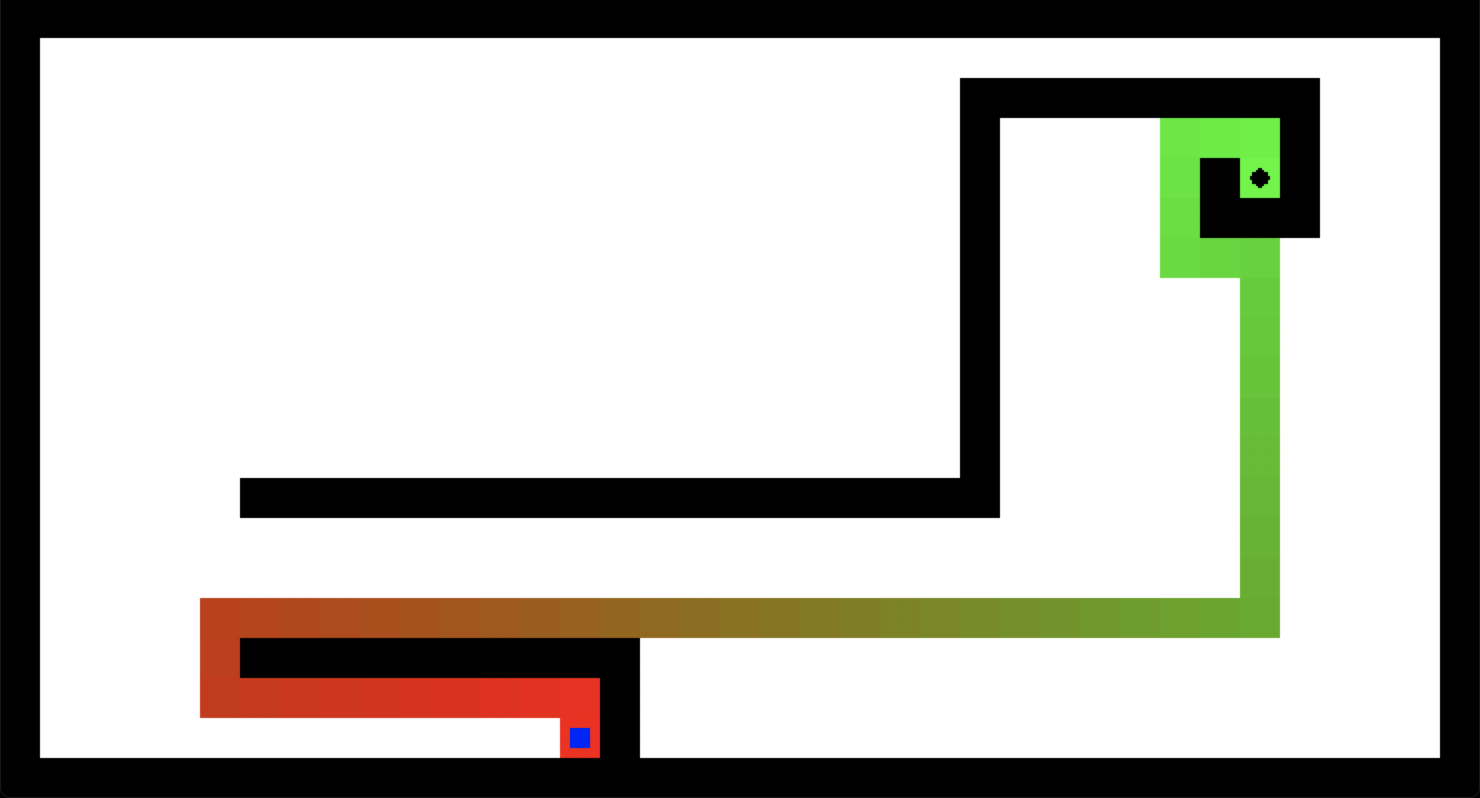
\includegraphics[width=12.5cm]{greedy_openmaze.png}
\end{center}
\begin{center}
\small{Figure 3.3.3. Greedy Solution for openMaze.txt}
\end{center}

\subsection{A*}



\subsubsection{mediumMaze.txt}
Path Length: 111 \\ \\
States Explored: 363
\begin{center}
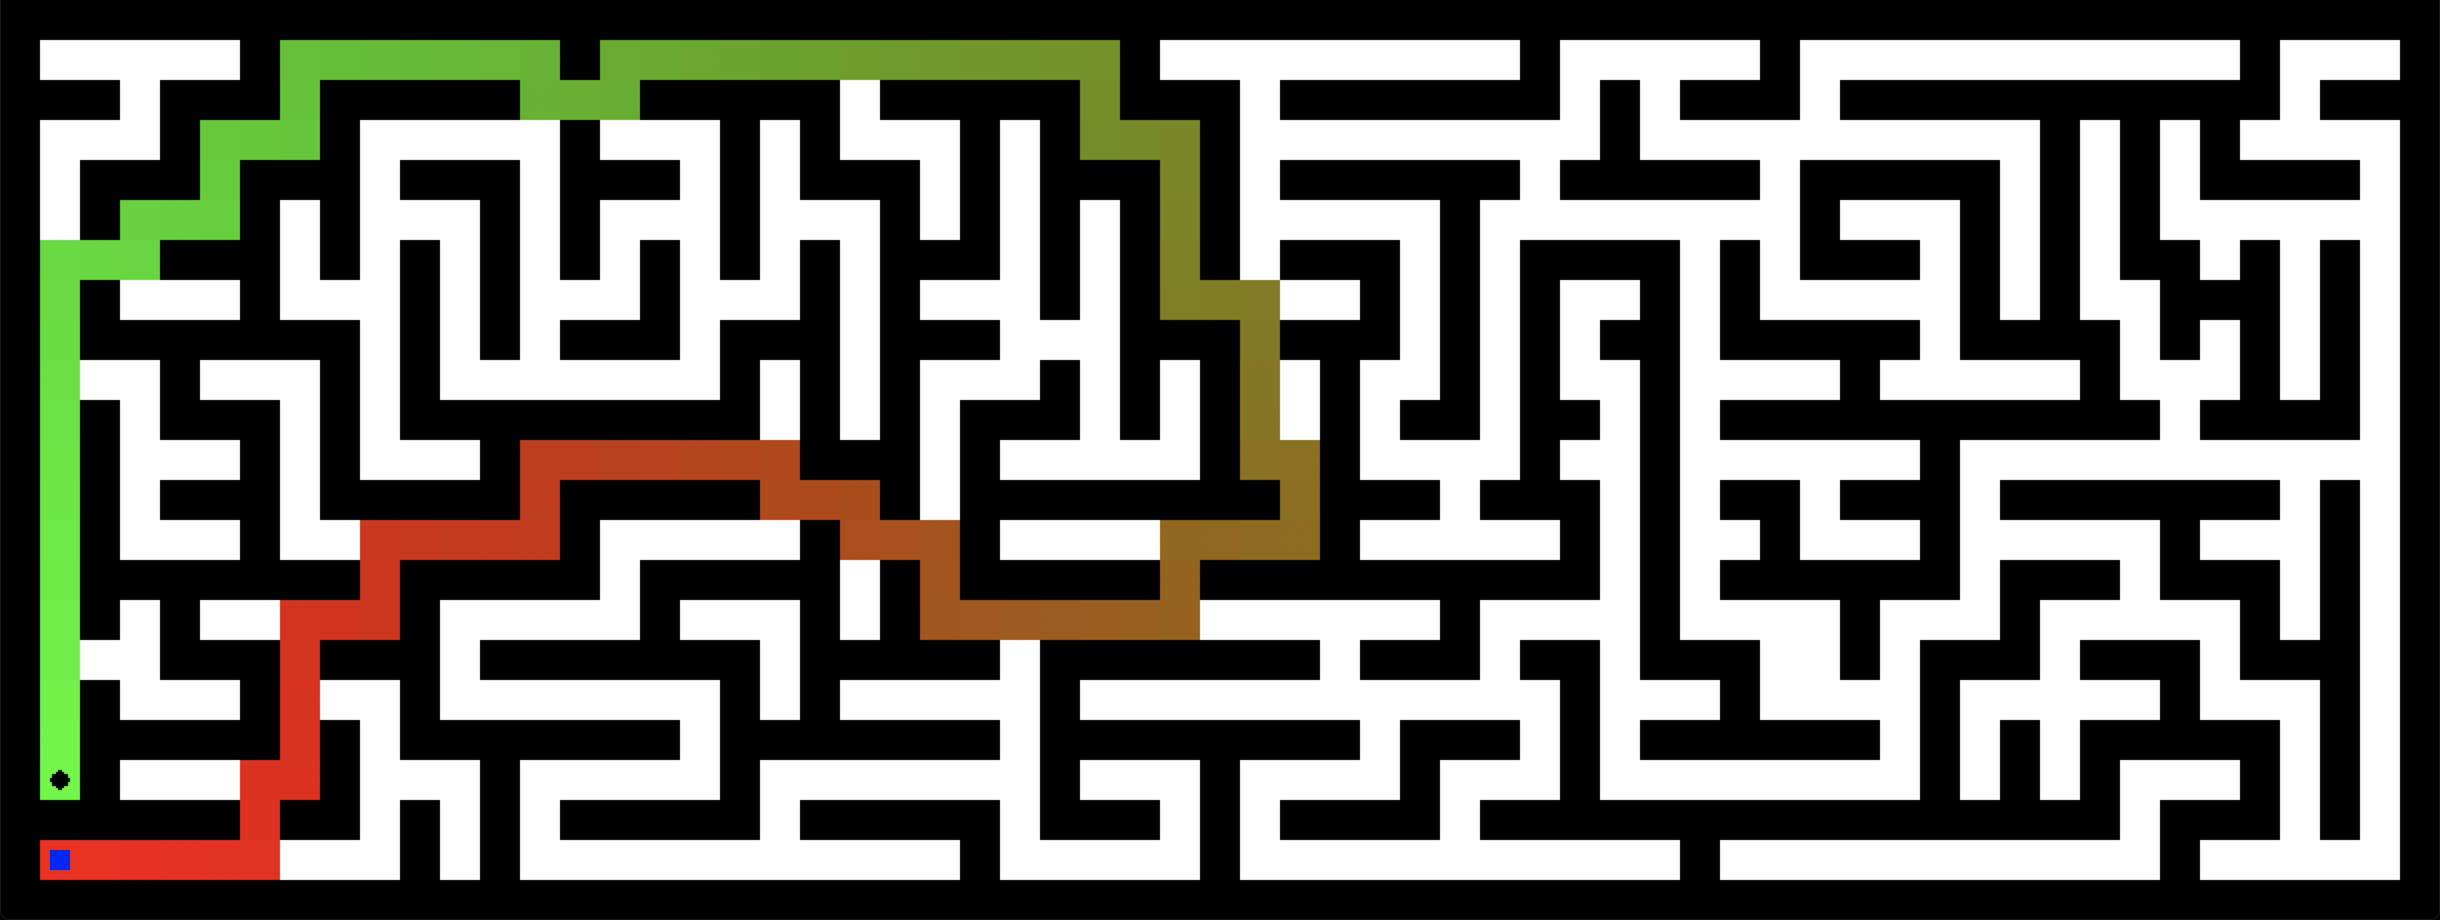
\includegraphics[width=15cm]{A_mediummaze.png}
\end{center}
\begin{center}
\small{Figure 3.4.1. A* Solution for mediumMaze.txt}
\end{center}

\subsubsection{bigMaze.txt}
Path Length: 183 \\ \\
States Explored: 1301
\begin{center}
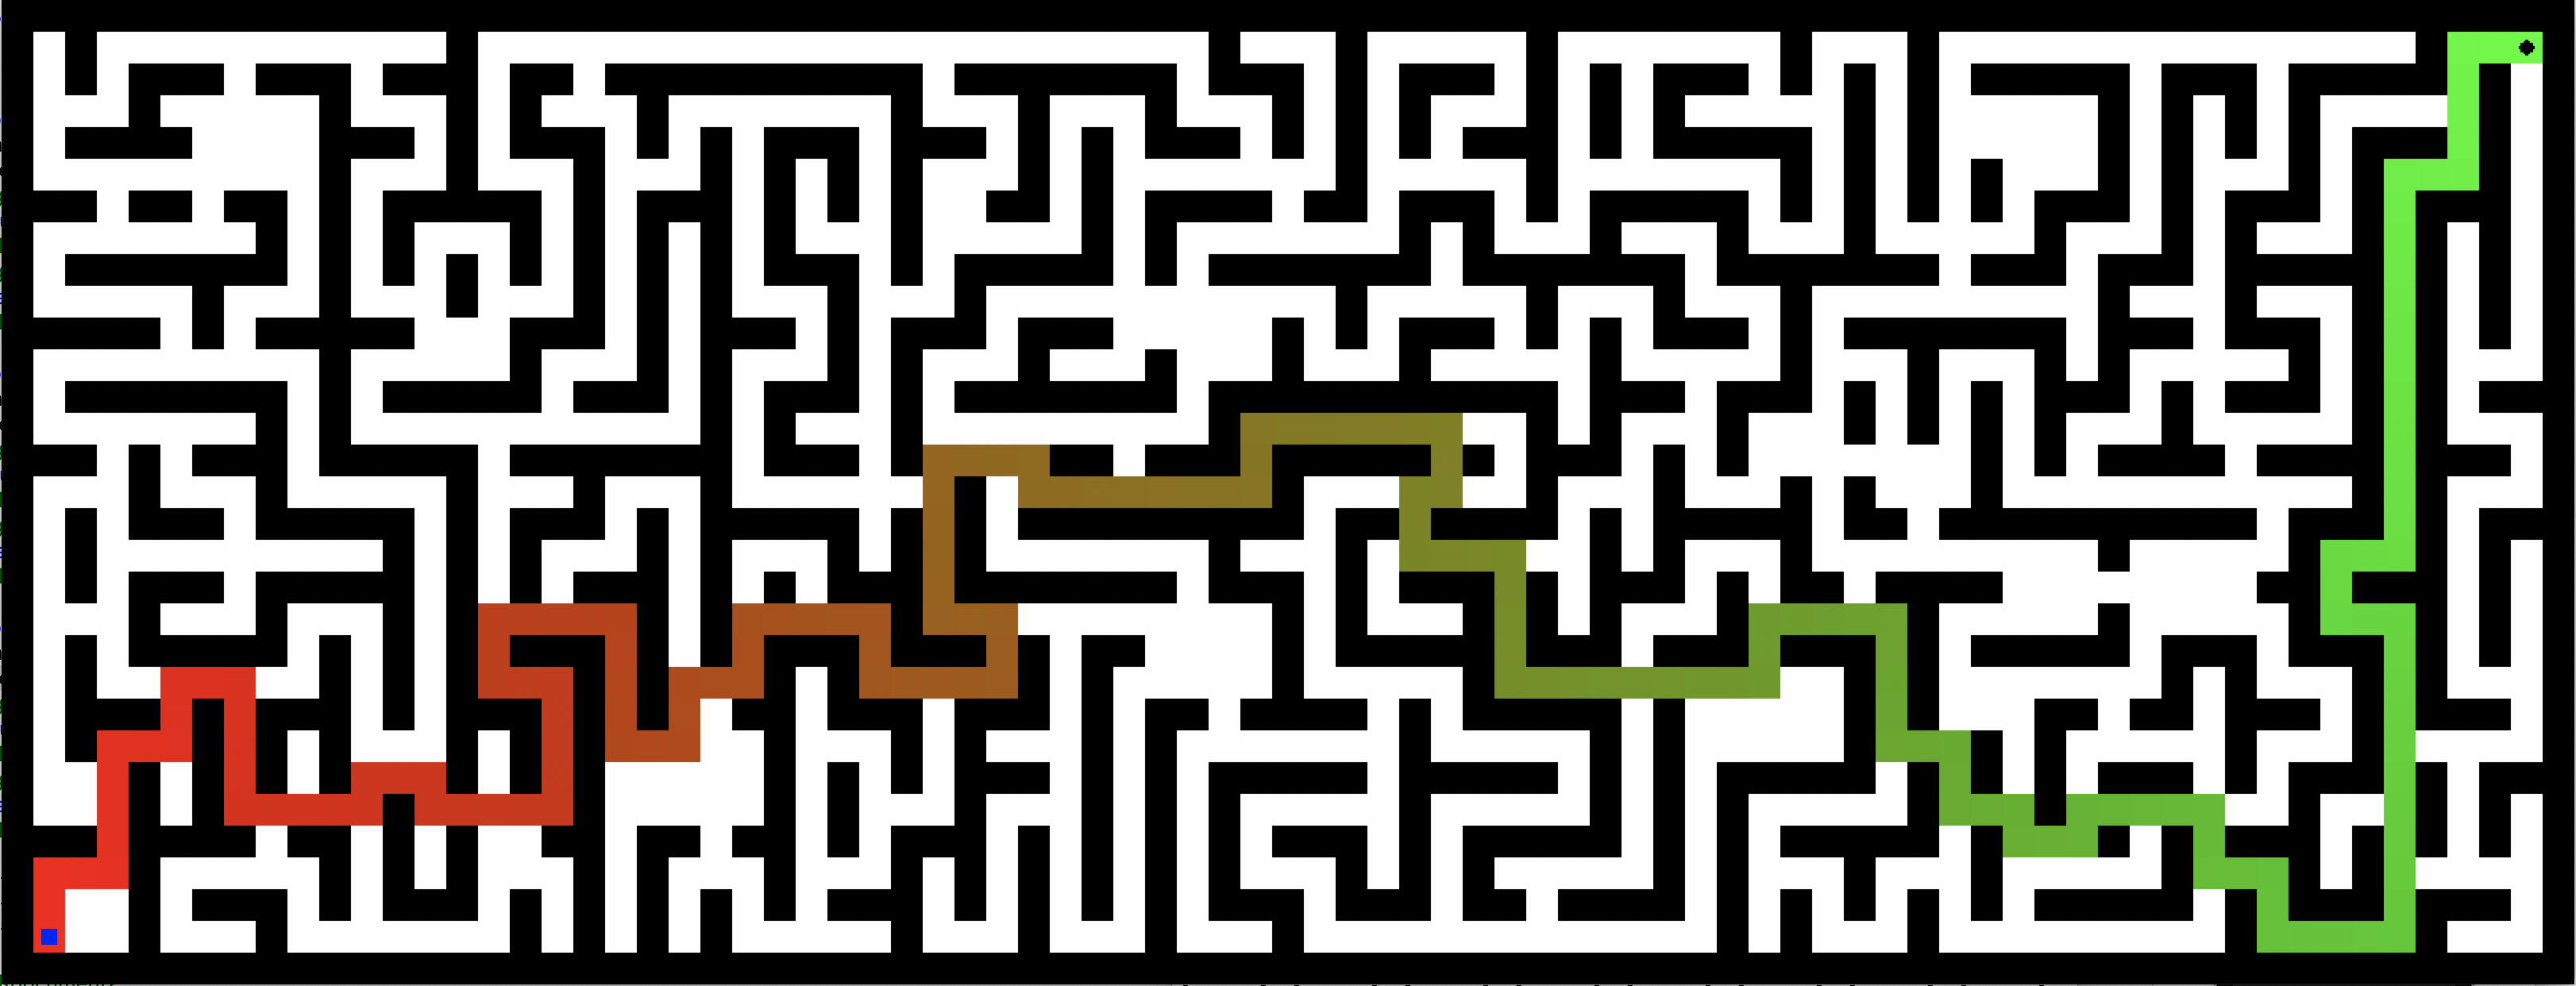
\includegraphics[width=15cm]{A_bigmaze.png}
\end{center}
\begin{center}
\small{Figure 3.4.2. A* Solution for bigMaze.txt}
\end{center}

\subsubsection{openMaze.txt}
Path Length: 52 \\ \\
States Explored: 384
\begin{center}
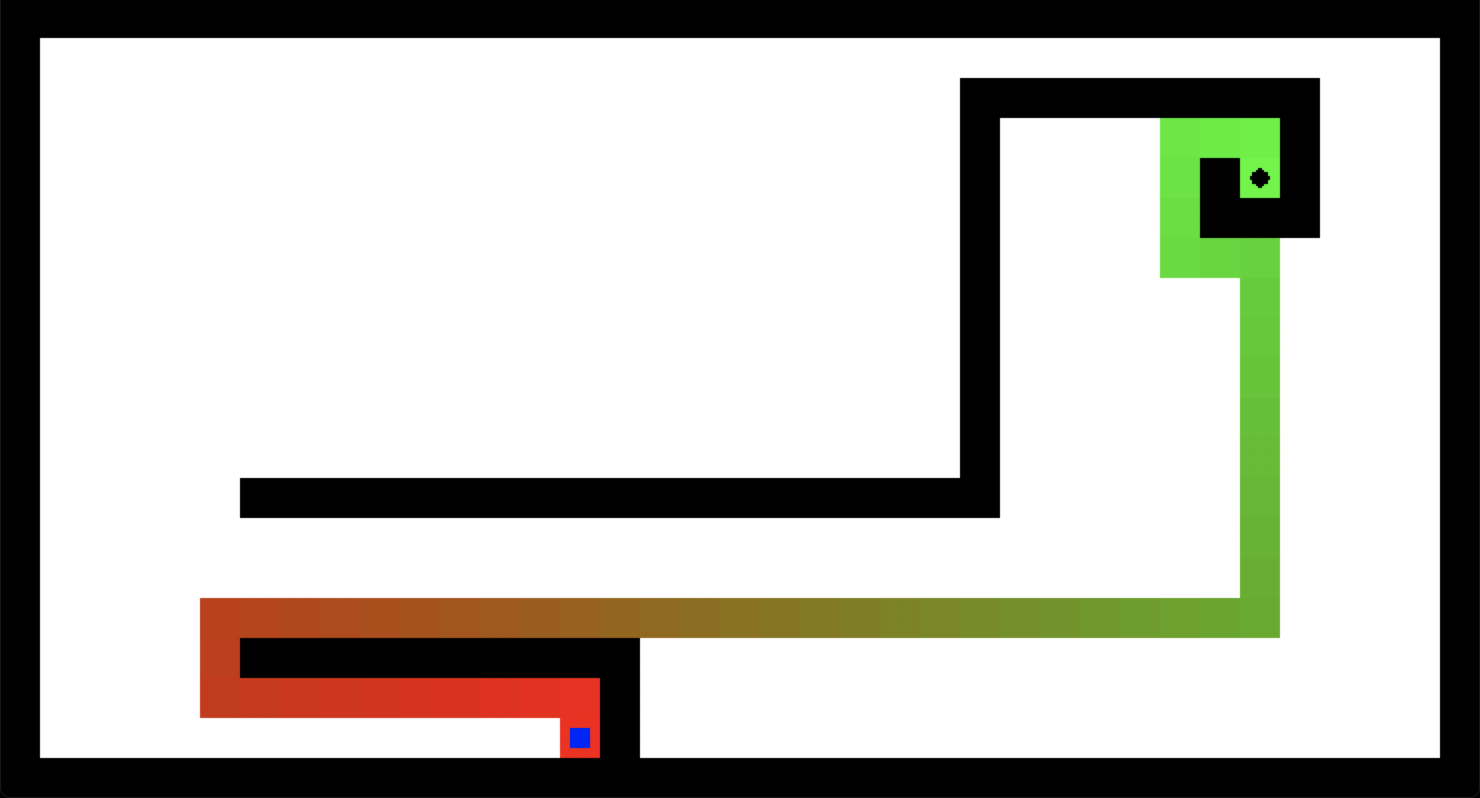
\includegraphics[width=12.5cm]{greedy_openmaze.png}
\end{center}
\begin{center}
\small{Figure 3.4.3. A* Solution for openMaze.txt}
\end{center}

\section{Section IV}

\subsection{tinySearch.txt}

Path Length: 38 \\ \\
States Explored: 830
\begin{center}
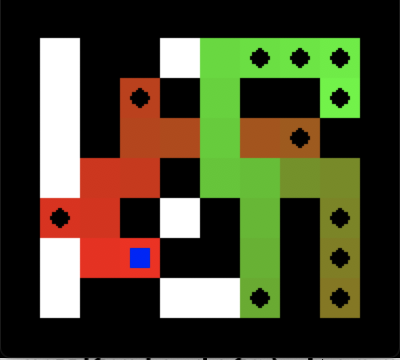
\includegraphics[width=6cm]{tiny.png}
\end{center}
\begin{center}
\small{Figure 4.1. A* Solution for tinySearch.txt}
\end{center}

\subsection{smallSearch.txt}
Path Length: 149 \\ \\
States Explored: 9261
\begin{center}

\includegraphics[width=15cm]{small.png}
\end{center}
\begin{center}
\small{Figure 4.2. A* Solution for smallSearch.txt}
\end{center}

\subsection{mediumSearch.txt}
Path Length: 209 \\ \\
States Explored: 24051
\begin{center}
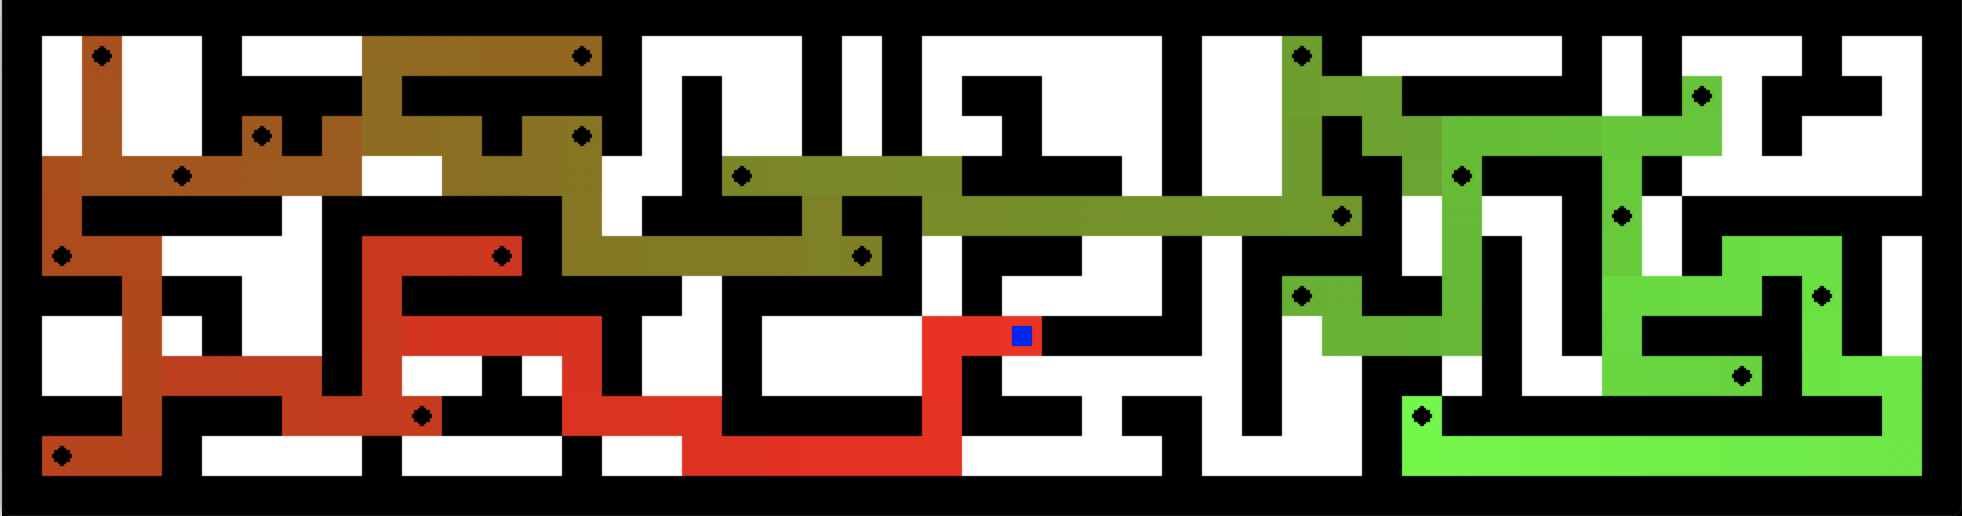
\includegraphics[width=15cm]{medium.png}
\end{center}
\begin{center}
\small{Figure 4.3. A* Solution for mediumSearch.txt}
\end{center}

\section{Statement of Contribution}
Jin Yucheng implemented BFS and DFS, Jin Hangtao also implemented BFS and DFS. Xie Yiqing implemented Greedy BFS and A*. The report is written by Jin Yucheng and Xie Yiqing.  

\end{document}

%% 
%% This work consists of these files mcmthesis.dtx,
%%                                   figures/ and
%%                                   code/,
%% and the derived files             mcmthesis.cls,
%%                                   mcmthesis-demo.tex,
%%                                   README,
%%                                   LICENSE,
%%                                   mcmthesis.pdf and
%%                                   mcmthesis-demo.pdf.
%%
%% End of file `mcmthesis-demo.tex'.
